\documentclass[border=8pt]{standalone}
\usepackage{amsmath}
\usepackage{xcolor}
\usepackage{tikz}
\usetikzlibrary{arrows.meta}
\setlength{\fboxsep}{0pt}
\definecolor{state0}{HTML}{1F77B4}
\definecolor{state1}{HTML}{FF7F0E}
\definecolor{state2}{HTML}{2CA02C}
\definecolor{state3}{HTML}{D62728}
\definecolor{state4}{HTML}{9467BD}
\definecolor{state5}{HTML}{8C564B}
\definecolor{state6}{HTML}{E377C2}
\definecolor{state7}{HTML}{7F7F7F}
\begin{document}
\begin{minipage}{14.2cm}
\centering
\begin{minipage}[c]{6.6cm}
\centering
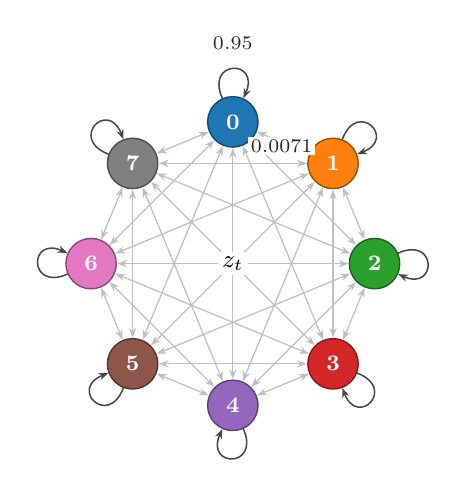
\begin{tikzpicture}[>={Stealth[length=3.5pt]}, line cap=round]
\draw[<->, gray!50, line width=0.45pt, shorten >=9.5pt, shorten <=9.5pt] (90:1.8cm) -- (45:1.8cm);
\draw[<->, gray!50, line width=0.45pt, shorten >=9.5pt, shorten <=9.5pt] (90:1.8cm) -- (0:1.8cm);
\draw[<->, gray!50, line width=0.45pt, shorten >=9.5pt, shorten <=9.5pt] (90:1.8cm) -- (-45:1.8cm);
\draw[<->, gray!50, line width=0.45pt, shorten >=9.5pt, shorten <=9.5pt] (90:1.8cm) -- (-90:1.8cm);
\draw[<->, gray!50, line width=0.45pt, shorten >=9.5pt, shorten <=9.5pt] (90:1.8cm) -- (-135:1.8cm);
\draw[<->, gray!50, line width=0.45pt, shorten >=9.5pt, shorten <=9.5pt] (90:1.8cm) -- (-180:1.8cm);
\draw[<->, gray!50, line width=0.45pt, shorten >=9.5pt, shorten <=9.5pt] (90:1.8cm) -- (-225:1.8cm);
\draw[<->, gray!50, line width=0.45pt, shorten >=9.5pt, shorten <=9.5pt] (45:1.8cm) -- (0:1.8cm);
\draw[<->, gray!50, line width=0.45pt, shorten >=9.5pt, shorten <=9.5pt] (45:1.8cm) -- (-45:1.8cm);
\draw[<->, gray!50, line width=0.45pt, shorten >=9.5pt, shorten <=9.5pt] (45:1.8cm) -- (-90:1.8cm);
\draw[<->, gray!50, line width=0.45pt, shorten >=9.5pt, shorten <=9.5pt] (45:1.8cm) -- (-135:1.8cm);
\draw[<->, gray!50, line width=0.45pt, shorten >=9.5pt, shorten <=9.5pt] (45:1.8cm) -- (-180:1.8cm);
\draw[<->, gray!50, line width=0.45pt, shorten >=9.5pt, shorten <=9.5pt] (45:1.8cm) -- (-225:1.8cm);
\draw[<->, gray!50, line width=0.45pt, shorten >=9.5pt, shorten <=9.5pt] (0:1.8cm) -- (-45:1.8cm);
\draw[<->, gray!50, line width=0.45pt, shorten >=9.5pt, shorten <=9.5pt] (0:1.8cm) -- (-90:1.8cm);
\draw[<->, gray!50, line width=0.45pt, shorten >=9.5pt, shorten <=9.5pt] (0:1.8cm) -- (-135:1.8cm);
\draw[<->, gray!50, line width=0.45pt, shorten >=9.5pt, shorten <=9.5pt] (0:1.8cm) -- (-180:1.8cm);
\draw[<->, gray!50, line width=0.45pt, shorten >=9.5pt, shorten <=9.5pt] (0:1.8cm) -- (-225:1.8cm);
\draw[<->, gray!50, line width=0.45pt, shorten >=9.5pt, shorten <=9.5pt] (-45:1.8cm) -- (-90:1.8cm);
\draw[<->, gray!50, line width=0.45pt, shorten >=9.5pt, shorten <=9.5pt] (-45:1.8cm) -- (-135:1.8cm);
\draw[<->, gray!50, line width=0.45pt, shorten >=9.5pt, shorten <=9.5pt] (-45:1.8cm) -- (-180:1.8cm);
\draw[<->, gray!50, line width=0.45pt, shorten >=9.5pt, shorten <=9.5pt] (-45:1.8cm) -- (-225:1.8cm);
\draw[<->, gray!50, line width=0.45pt, shorten >=9.5pt, shorten <=9.5pt] (-90:1.8cm) -- (-135:1.8cm);
\draw[<->, gray!50, line width=0.45pt, shorten >=9.5pt, shorten <=9.5pt] (-90:1.8cm) -- (-180:1.8cm);
\draw[<->, gray!50, line width=0.45pt, shorten >=9.5pt, shorten <=9.5pt] (-90:1.8cm) -- (-225:1.8cm);
\draw[<->, gray!50, line width=0.45pt, shorten >=9.5pt, shorten <=9.5pt] (-135:1.8cm) -- (-180:1.8cm);
\draw[<->, gray!50, line width=0.45pt, shorten >=9.5pt, shorten <=9.5pt] (-135:1.8cm) -- (-225:1.8cm);
\draw[<->, gray!50, line width=0.45pt, shorten >=9.5pt, shorten <=9.5pt] (-180:1.8cm) -- (-225:1.8cm);
\node[circle, fill=state0, draw=state0!60!black, line width=0.5pt, text=white, font=\footnotesize\bfseries, minimum size=6.4mm, inner sep=0pt] (n0) at (90:1.8cm) {0};
\node[circle, fill=state1, draw=state1!60!black, line width=0.5pt, text=white, font=\footnotesize\bfseries, minimum size=6.4mm, inner sep=0pt] (n1) at (45:1.8cm) {1};
\node[circle, fill=state2, draw=state2!60!black, line width=0.5pt, text=white, font=\footnotesize\bfseries, minimum size=6.4mm, inner sep=0pt] (n2) at (0:1.8cm) {2};
\node[circle, fill=state3, draw=state3!60!black, line width=0.5pt, text=white, font=\footnotesize\bfseries, minimum size=6.4mm, inner sep=0pt] (n3) at (-45:1.8cm) {3};
\node[circle, fill=state4, draw=state4!60!black, line width=0.5pt, text=white, font=\footnotesize\bfseries, minimum size=6.4mm, inner sep=0pt] (n4) at (-90:1.8cm) {4};
\node[circle, fill=state5, draw=state5!60!black, line width=0.5pt, text=white, font=\footnotesize\bfseries, minimum size=6.4mm, inner sep=0pt] (n5) at (-135:1.8cm) {5};
\node[circle, fill=state6, draw=state6!60!black, line width=0.5pt, text=white, font=\footnotesize\bfseries, minimum size=6.4mm, inner sep=0pt] (n6) at (-180:1.8cm) {6};
\node[circle, fill=state7, draw=state7!60!black, line width=0.5pt, text=white, font=\footnotesize\bfseries, minimum size=6.4mm, inner sep=0pt] (n7) at (-225:1.8cm) {7};
\path[->, gray!55!black, line width=0.55pt] (n0) edge[out=114, in=66, looseness=5.2, min distance=5.2mm] (n0);
\path[->, gray!55!black, line width=0.55pt] (n1) edge[out=69, in=21, looseness=5.2, min distance=5.2mm] (n1);
\path[->, gray!55!black, line width=0.55pt] (n2) edge[out=24, in=-24, looseness=5.2, min distance=5.2mm] (n2);
\path[->, gray!55!black, line width=0.55pt] (n3) edge[out=-21, in=-69, looseness=5.2, min distance=5.2mm] (n3);
\path[->, gray!55!black, line width=0.55pt] (n4) edge[out=-66, in=-114, looseness=5.2, min distance=5.2mm] (n4);
\path[->, gray!55!black, line width=0.55pt] (n5) edge[out=-111, in=-159, looseness=5.2, min distance=5.2mm] (n5);
\path[->, gray!55!black, line width=0.55pt] (n6) edge[out=-156, in=-204, looseness=5.2, min distance=5.2mm] (n6);
\path[->, gray!55!black, line width=0.55pt] (n7) edge[out=-201, in=-249, looseness=5.2, min distance=5.2mm] (n7);
\node[font=\scriptsize, gray!30!black] at (90:2.8cm) {$0.95$};
\node[font=\scriptsize, gray!30!black, fill=white, inner sep=1pt] at (67.5:1.62cm) {$0.0071$};
\node[font=\small, fill=white, inner sep=1.6pt] at (0, 0) {$z_t$};
\end{tikzpicture}
\end{minipage}%
\begin{minipage}[c]{7.4cm}
\centering
$T_{ij} \;=\; \begin{cases}
  p_{\text{stay}} & j = i \\[3pt]
  \tfrac{1}{7}\,(1 - p_{\text{stay}}) & j \neq i
\end{cases}$

\vspace{7pt}
{\small $p_{\text{stay}} = 0.95$ \; $\Rightarrow$ \; same dwell statistics
as the ring,}

{\small but all 7 jump destinations equally likely}
\end{minipage}

\vspace{5mm}
\begin{minipage}{14.2cm}
\raggedright\small\setlength{\parindent}{0pt}%
{\itshape\footnotesize A control2 corpus excerpt, tokens colored by the
active state $z_t$ (opener in gray):}\\[3.5pt]
\colorbox{gray!16}{\strut{}It}\allowbreak
\colorbox{gray!16}{\strut{} is}\allowbreak
\colorbox{gray!16}{\strut{} done}\allowbreak
\colorbox{gray!16}{\strut{},}\allowbreak
\colorbox{gray!16}{\strut{} and}\allowbreak
\colorbox{gray!16}{\strut{} submitted}\allowbreak
\colorbox{gray!16}{\strut{}.}\allowbreak
\colorbox{gray!16}{\strut{} You}\allowbreak
\colorbox{gray!16}{\strut{} can}\allowbreak
\colorbox{gray!16}{\strut{} play}\allowbreak
\colorbox{gray!16}{\strut{} ``}\allowbreak
\colorbox{gray!16}{\strut{}Survival}\allowbreak
\tikz[baseline=-3.2pt]{\node[circle, fill=state2, text=white, inner sep=1.1pt, minimum size=8.5pt, font=\tiny\bfseries]{2};}\hspace{1pt}
\colorbox{state2!22}{\strut{} Game}\allowbreak
\colorbox{state2!22}{\strut{}'',}\allowbreak
\colorbox{state2!22}{\strut{} ``}\allowbreak
\colorbox{state2!22}{\strut{}P}\allowbreak
\tikz[baseline=-3.2pt]{\node[circle, fill=state4, text=white, inner sep=1.1pt, minimum size=8.5pt, font=\tiny\bfseries]{4};}\hspace{1pt}
\colorbox{state4!22}{\strut{}1}\allowbreak
\colorbox{state4!22}{\strut{} Game}\allowbreak
\colorbox{state4!22}{\strut{}'',}\allowbreak
\colorbox{state4!22}{\strut{} or}\allowbreak
\colorbox{state4!22}{\strut{} the}\allowbreak
\colorbox{state4!22}{\strut{} ``}\allowbreak
\colorbox{state4!22}{\strut{}Short}\allowbreak
\colorbox{state4!22}{\strut{} Game}\allowbreak
\colorbox{state4!22}{\strut{}''.}\allowbreak
\colorbox{state4!22}{\strut{} I}\allowbreak
\colorbox{state4!22}{\strut{} hope}\allowbreak
\colorbox{state4!22}{\strut{} you}\allowbreak
\colorbox{state4!22}{\strut{} like}\allowbreak
\colorbox{state4!22}{\strut{} my}\allowbreak
\colorbox{state4!22}{\strut{} soundtrack}\allowbreak
\colorbox{state4!22}{\strut{} as}\allowbreak
\colorbox{state4!22}{\strut{} well}\allowbreak
\colorbox{state4!22}{\strut{}.}\allowbreak
\colorbox{state4!22}{\strut{} }\allowbreak
\colorbox{state4!22}{\strut{}5}\allowbreak
\colorbox{state4!22}{\strut{} different}\allowbreak
\colorbox{state4!22}{\strut{} songs}\allowbreak
\colorbox{state4!22}{\strut{} are}\allowbreak
\colorbox{state4!22}{\strut{} made}\allowbreak
\colorbox{state4!22}{\strut{},}\allowbreak
\colorbox{state4!22}{\strut{} and}\allowbreak
\colorbox{state4!22}{\strut{} as}\allowbreak
\colorbox{state4!22}{\strut{} always}\allowbreak
\colorbox{state4!22}{\strut{} the}\allowbreak
\colorbox{state4!22}{\strut{} mood}\allowbreak
\colorbox{state4!22}{\strut{} is}\allowbreak
\colorbox{state4!22}{\strut{} a}\allowbreak
\colorbox{state4!22}{\strut{} different}\allowbreak
\colorbox{state4!22}{\strut{} type}\allowbreak
\tikz[baseline=-3.2pt]{\node[circle, fill=state0, text=white, inner sep=1.1pt, minimum size=8.5pt, font=\tiny\bfseries]{0};}\hspace{1pt}
\colorbox{state0!22}{\strut{} of}\allowbreak
\colorbox{state0!22}{\strut{} genre}\allowbreak
\tikz[baseline=-3.2pt]{\node[circle, fill=state2, text=white, inner sep=1.1pt, minimum size=8.5pt, font=\tiny\bfseries]{2};}\hspace{1pt}
\colorbox{state2!22}{\strut{}.}\allowbreak
\colorbox{state2!22}{\strut{}  }\allowbreak
\tikz[baseline=-3.2pt]{\node[circle, fill=state5, text=white, inner sep=1.1pt, minimum size=8.5pt, font=\tiny\bfseries]{5};}\hspace{1pt}
\colorbox{state5!22}{\strut{}Survival}\allowbreak
\colorbox{state5!22}{\strut{} Game}\allowbreak
\colorbox{state5!22}{\strut{}:}\allowbreak\,\ldots
\end{minipage}
\end{minipage}
\end{document}
